\subsection{Expérience Apex}
\label{subsec:experience}

\subsubsection{Exigences et besoins}

L'objectif du système expérimental de la fusée est de déterminer la trajectoire de chaque étage en temps réel. De cet
objectif découlent trois besoins principaux.

\begin{itemize}
    \item \textbf{Disposer d'un système intégrable dans les deux étages}, il doit donc être compact, léger et consommer peu
    d'énergie.
    \item \textbf{Mesurer un nombre suffisant de paramètres}, afin de réduire l'incertitude sur l'estimation de la
    trajectoire. Les paramètres retenus sont les suivants :
    \begin{itemize}
        \item l'accélération linéaire ;
        \item la vitesse angulaire ;
        \item le champ magnétique ;
        \item la pression statique ;
        \item la température ;
        \item les données GNSS.
    \end{itemize}
    Pour le deuxième étage, la pression totale au niveau de la pointe de la coiffe est également mesurée. L'ensemble de ces
    mesures, associé à d'autre variables interne, constitue un enregistrement de \SI{127}{\byte}\footnote{\label{fn:byte}
    \SI{}{\byte} pour byte(s) ou octet(s) en français} produit à une cadence de \SI{100}{\hertz}, soit un flux de
    \SI{12.7}{\kilo\byte\per\second}\footnoteref{fn:byte} (\SI{101.6}{\kilo bit\per\second}).\\

    \item \textbf{Disposer de points d'observabilité suffisants}, afin de pouvoir recalculer la trajectoire après le vol et
    la comparer à celle déterminée en vol. L'objectif est de récupérer l'intégralité du flux de données du calculateur, à la
    fréquence de l'algorithme de calcul. Pour chaque étage, deux cas se présentent :
    \begin{itemize}
        \item l'étage est retrouvé intact : un moyen de sauvegarde numérique embarquée pouvant contenir l'intégralité du flux sur
        la durée du vol, soit moins de \SI{4}{\mega\byte}\footnoteref{fn:byte} pour un vol de cinq minutes, doit être prévu ;
        \item l'étage n'est pas retrouvé ou dans un état ne permettant pas la récupération des données enregistrées : la seule
        manière de disposer malgré tout du flux est de l'avoir émis pendant le vol, ce qui impose un moyen de télémesure à bord et
        une station de réception au sol.
    \end{itemize}
    Le besoin d'observabilité est donc avant tout un besoin post-vol. La télémesure n'est requise que comme garantie contre la
    perte d'un étage ; mais dès lors que ce flux est émis en vol, il devient possible de suivre la trajectoire en direct depuis
    le sol. Cela constitue une opportunité que le système expérimental exploite.\\
\end{itemize}

Cependant, la fusée n'est pas un système passif : le premier étage déploie des aérofreins puis commande la séparation avec le
deuxième étage, ce dernier peut ou non déclencher son propulseur, et chaque étage déploie son parachute. Bien que le déroulement
de la mission soit assuré par les séquenceurs, le système expérimental doit connaître la chronologie de ces actions, puisqu'elles
influent directement sur la trajectoire des étages.\\

Par ailleurs, la détermination de l'attitude de la fusée par le séquenceur à partir du capteur \verb|wt901b| ne relève pas de
l'expérience : elle est nécessaire au déroulement du vol. Elle constitue néanmoins une première pour l'équipe, tant par la méthode
employée que par l'utilisation de ce type de capteur, ce qui justifie de la valider expérimentalement.\\

Ces deux constats se traduisent par deux besoins supplémentaires :
\begin{itemize}
    \item connaître les actions exécutées par les séquenceurs, ainsi que leur datation ;
    \item être capable de valider la technique de détermination de l'attitude mise en œuvre par les séquenceurs.\\
\end{itemize}

\newpage

\subsubsection{Module Apex et limitations}

En prenant en compte l'ensemble de ces besoins, il a été déterminé que le module \gls{APEX}, déjà existant et fonctionnel en deux
exemplaires, constituait une base solide pour le système expérimental. Il a donc été décidé de l'utiliser comme module
expérimental principale, avec quelques améliorations. En effet, le module pocède : \\

\hspace*{-\parindent}%
\begin{minipage}{0.65\textwidth}
    \begin{itemize}
        \item Un microcontroleur \verb|STM32F411RETx| ;
        \item Une mémoire flash de \SI{64}{\mega\byte} ;
        \item Trois accéléromètres ayant des plages de mesures différentes ;
        \item Un gyromètre ;
        \item Un magnétomètre ;
        \item Un baromètre ;
        \item Un capteur de température ;
        \item Un récepteur \acrshort{GNSS} ;
        \item Un module de télémesure \verb|rfm95w| .
    \end{itemize}
    La référence suivante \cite{APEX} donne accès à la documentation complète du module \gls{APEX}.\\
    Le module possède également un connecteur de 20 pins permettant de fortement d'étendre ses fonctionnalités. En effet, seul,
    la carte ne remplie pas tous les besoins exprimés précédemment.
\end{minipage}
\hfill
\begin{minipage}{0.3\textwidth}
    \begin{figure}[H]
        \centering
        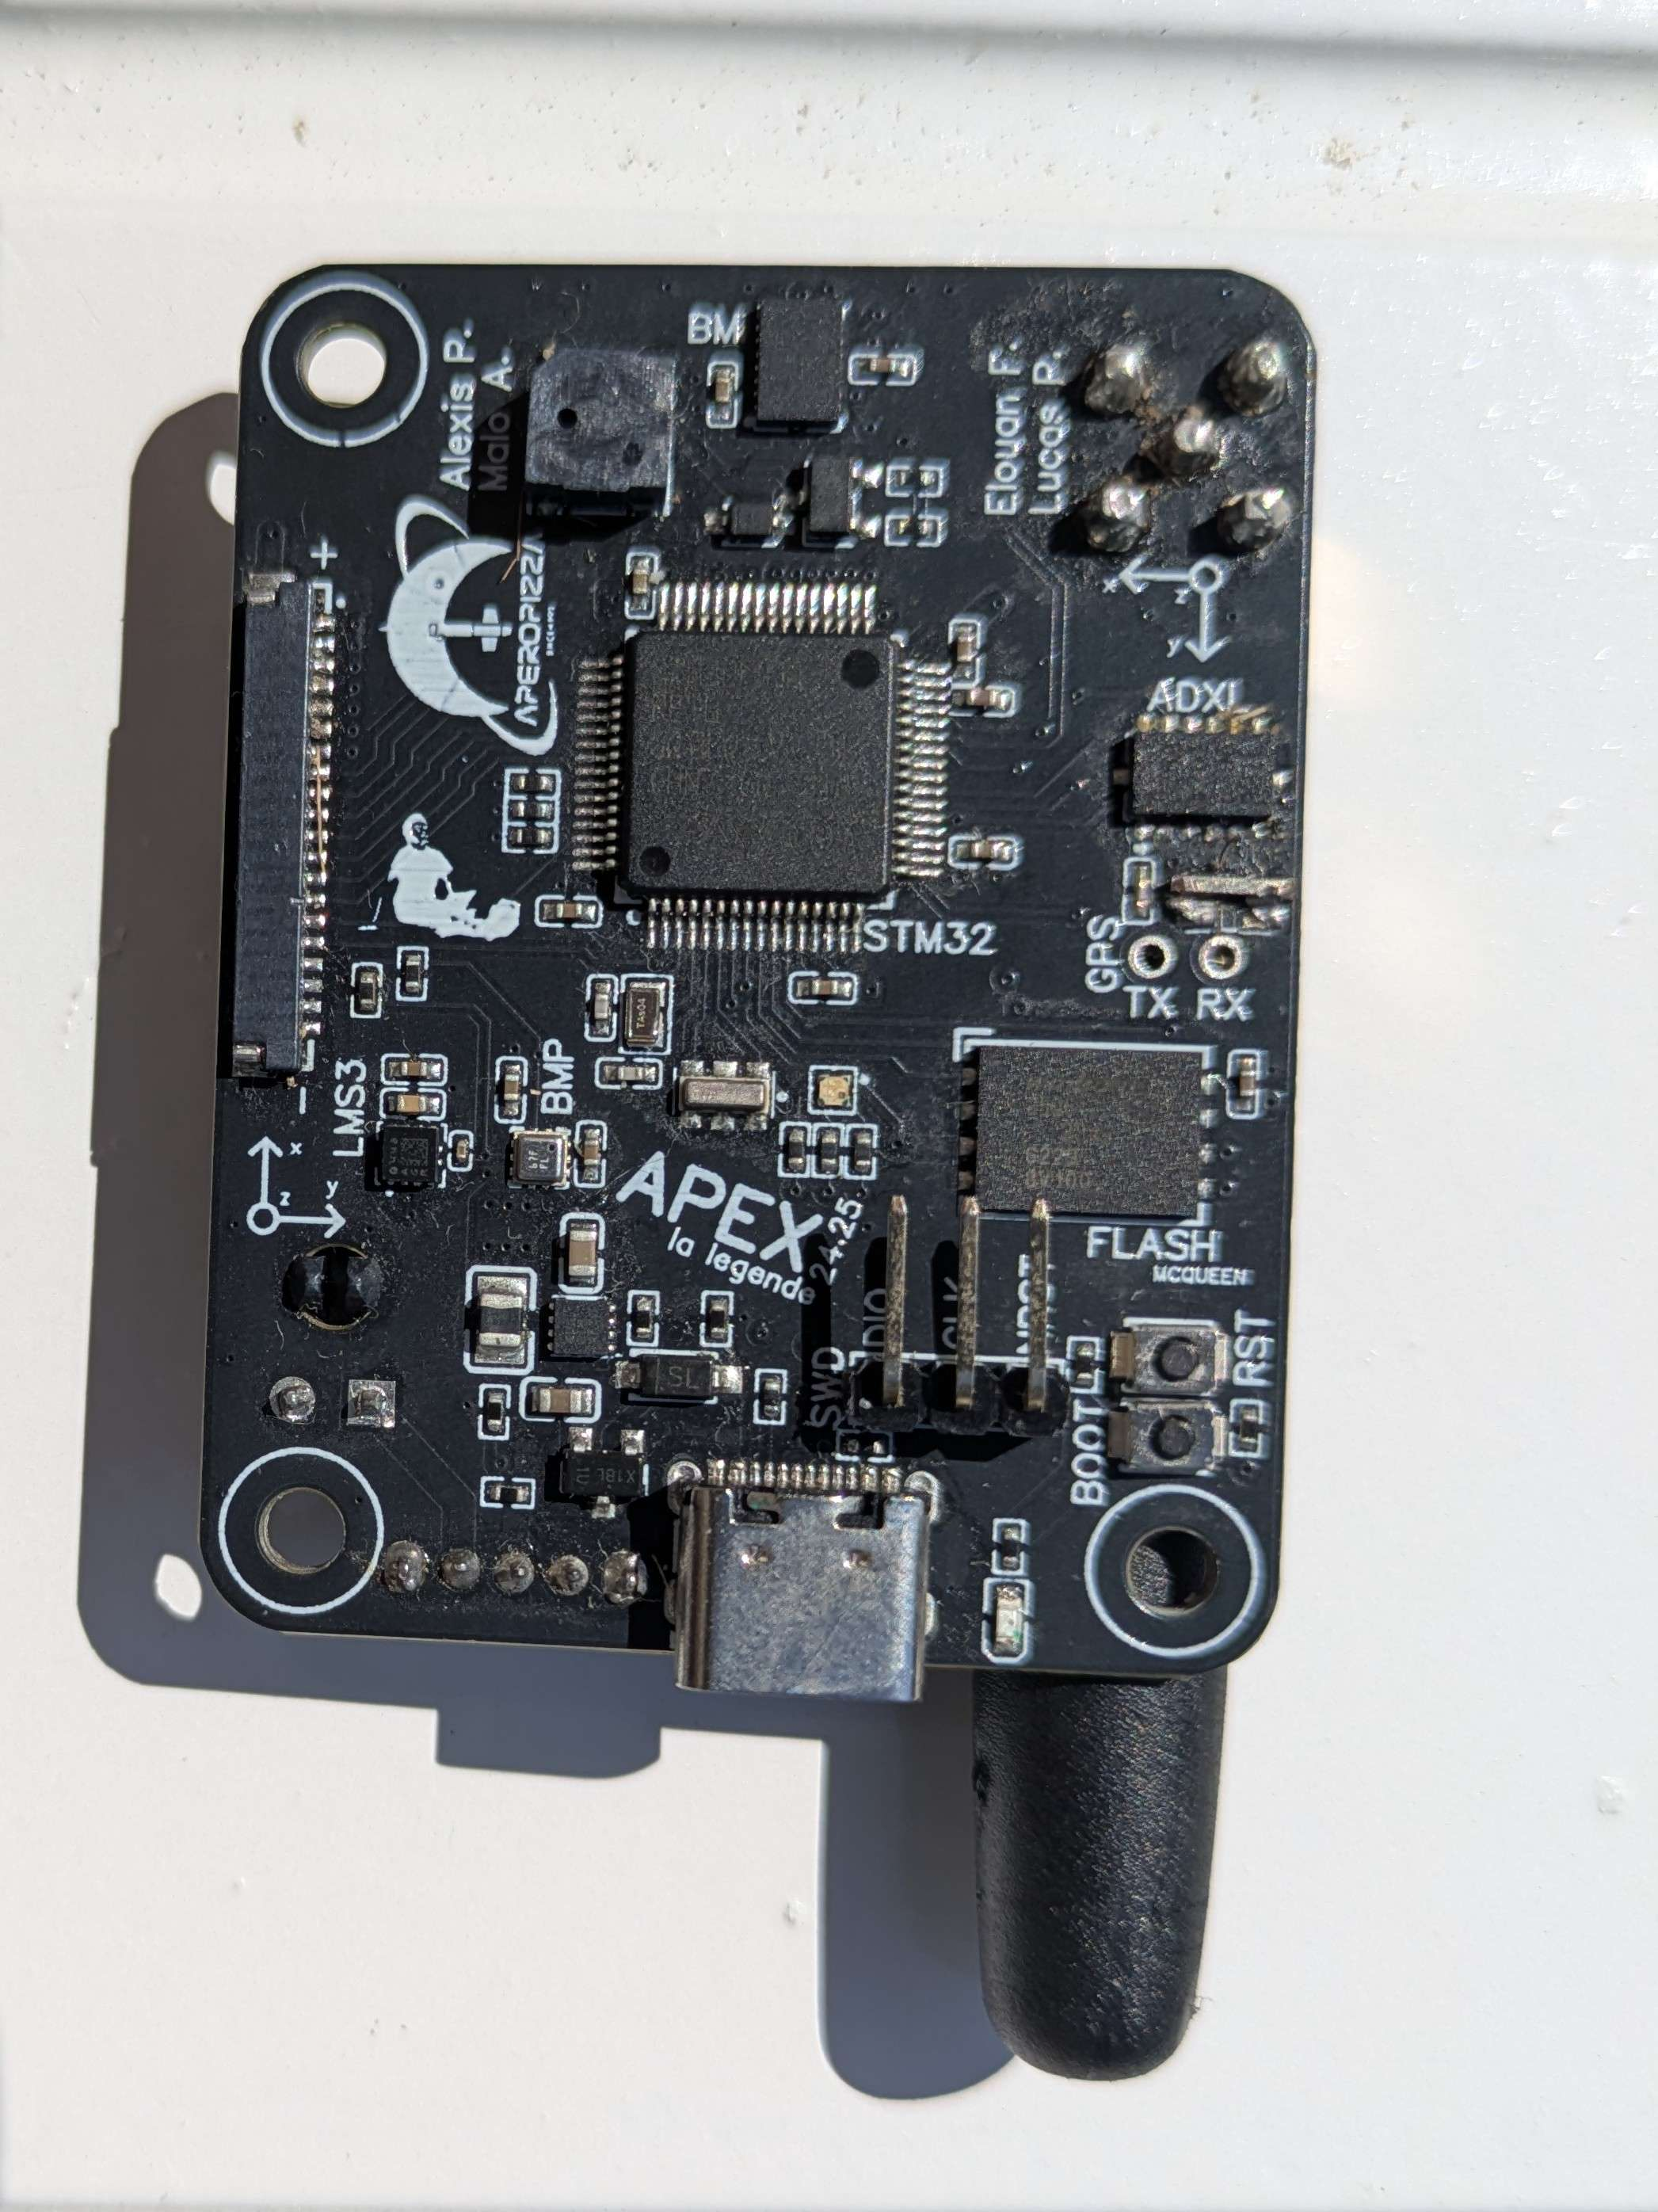
\includegraphics[width=\textwidth]{figures/elec/APEX_FRONT.jpg}
        \caption{Vue de face du module \gls{APEX}.}
        \label{fig:apex_front}
    \end{figure}
\end{minipage}

\vspace{0.5cm}

L'un des retours d'expérience des équipes ayant précédemment travaillés sur les modules Unknown et Apex est que le choix du système
de télémesure est crucial et nécessite de faire des compromis. L'un des protocoles de télémesure les plus répandus est le
\acrshort{LORA}, qui permet d'émettre un flux de données sur de longues distance et à faible consommation. Cependant, le débit de
ce protocole est limité à une dizaines de kilobits par seconde, ce qui est bien en deçà du flux de données produit par le module
expérimental.\\

Un autre protocole de télémesure grandement utilisé dans le domaine de l'astromodélisme est le \acrshort{FSK}. Il
permet d'émettre un flux de données à des débits bien plus élevés que le \acrshort{LORA}, mais à des distances bien inférieures
pour une même puissance d'émission.\\

Le choix d'utiliser les deux protocoles de télémesures a donc été fait : 
\begin{itemize}
    \item Le protocole \acrshort{FSK} est utilisé pour émettre le flux de données du module expérimental, afin de suivre la
    trajectoire en direct depuis le sol ;
    \item Le protocole \acrshort{LORA} est utilisé pour émettre un flux de données plus léger, contenant les informations
    essentielles de la fusée comme par exemple la position \acrshort{GPS}.
\end{itemize}

\newpage

\subsubsection{Module ApexEx}

Afin de couvrir l'ensemble des besoins exprimés, il a été décidé de concevoir une carte supplémentaire, nommée ApexEx (Apex
Extension). Cette carte sera connectée au module \gls{APEX} via le connecteur de 20 pins.

\begin{figure}[H]
    \centering
    \begin{subfigure}{0.49\textwidth}
        \centering
        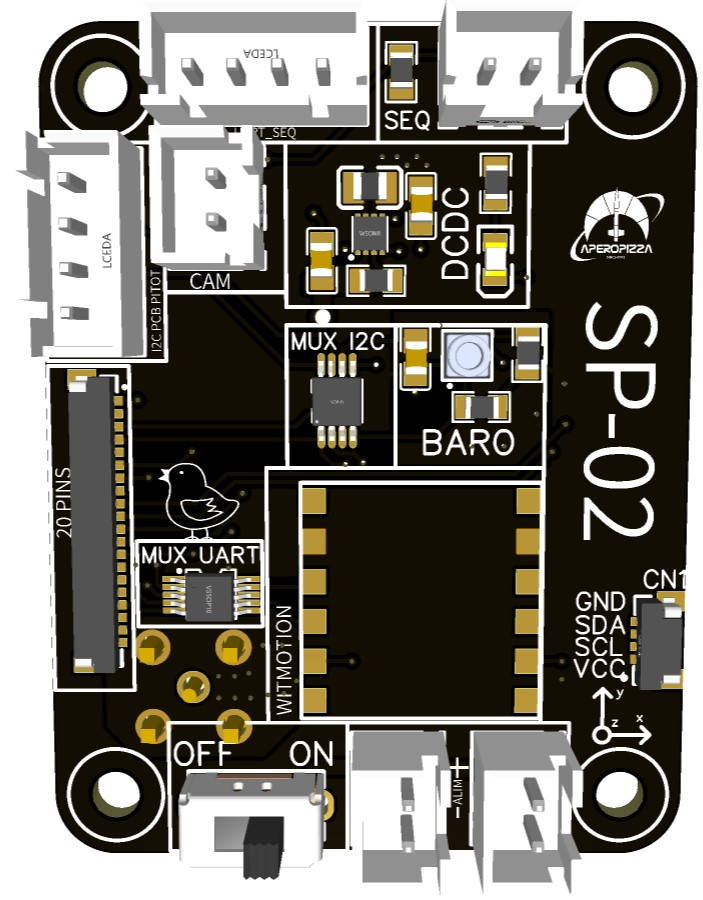
\includegraphics[width=0.6\textwidth]{figures/elec/PCB_ApexEx_FRONT.jpg}
        \caption{Vue de face du module ApexEx.}
        \label{fig:apexex_front}
    \end{subfigure}
    \hfill
    \begin{subfigure}{0.49\textwidth}
        \centering
        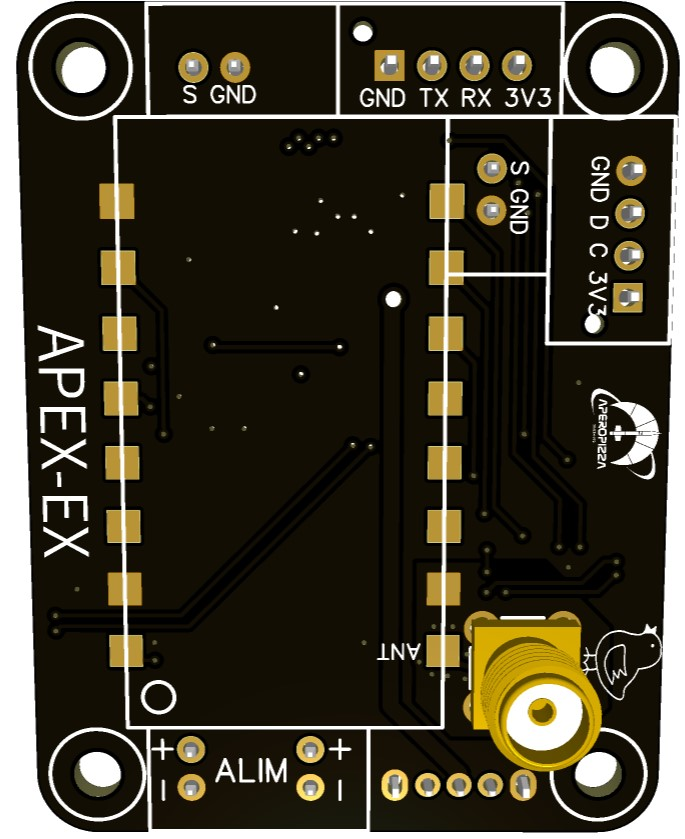
\includegraphics[width=0.6\textwidth]{figures/elec/PCB_ApexEx_BACK.jpg}
        \caption{Vue de dos du module ApexEx.}
        \label{fig:apexex_back}
    \end{subfigure}
    \caption{Vue du module ApexEx.}
    \label{fig:apexex}
\end{figure}

Ce nouveau module ne possède pas de microcontroleur, la logique de contrôle étant assurée par le module \gls{APEX}.
Il permet d'ajouter les fonctionnalités suivantes au système expérimental : \\

\hspace*{-\parindent}%
\begin{minipage}{0.45\textwidth}
    \begin{itemize}
        \item Un baromètre \verb|ILP28SQSW| ;
        \item Un module \verb|wt901b| ;
        \item Un transceiver radio \verb|LORA1276F30| ;
        \item Un ensemble de deux connecteurs reliant le module d'expérience de l'étage courant au séquenceur s'y trouvant ;
        \item Un connecteur branché à un deuxième baromètre \verb|ILP28SQSW| placé sur la carte Pitot se trouvant au niveau de la
        pointe de la coiffe du deuxième étage ;
        \item Un connecteur relié au système de caméra embarqué ;
        \item Un module de régulation de tension \verb|TPS62172|, le module \gls{APEX} ne fournissant pas de puissance via le
        connecteur de 20 pins.
    \end{itemize}
\end{minipage}
\hfill
\begin{minipage}{0.5\textwidth}
    \begin{figure}[H]
        \centering
        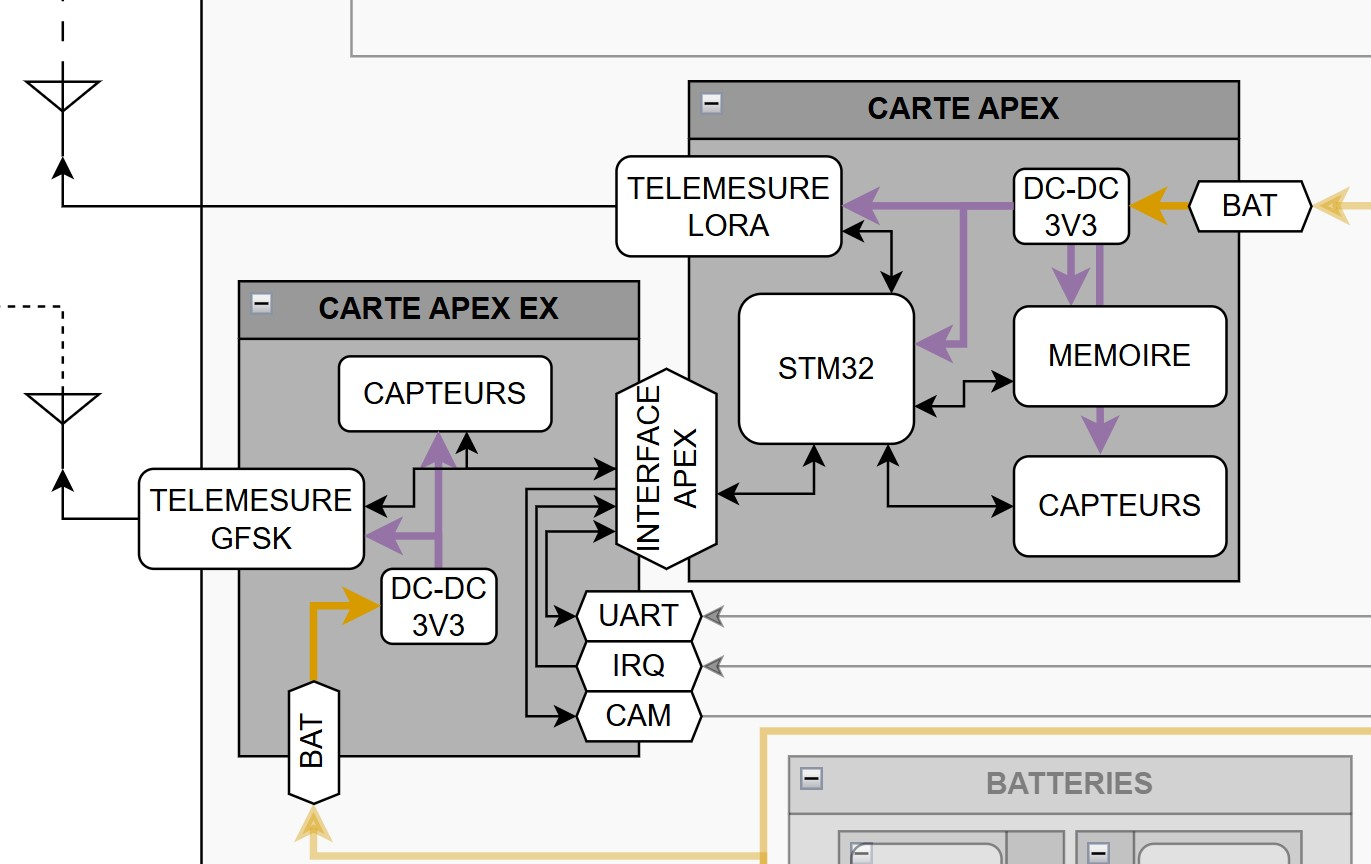
\includegraphics[width=\textwidth]{figures/elec/zoom_syno_apex.jpg}
        \caption{Zoom sur le synoptique du module expérimental (ref. annexe \ref{subsec:synoptique_fusee})}
        \label{fig:zoom_syno_apex}
    \end{figure}
\end{minipage}

\begin{figure}[H]
    \centering
    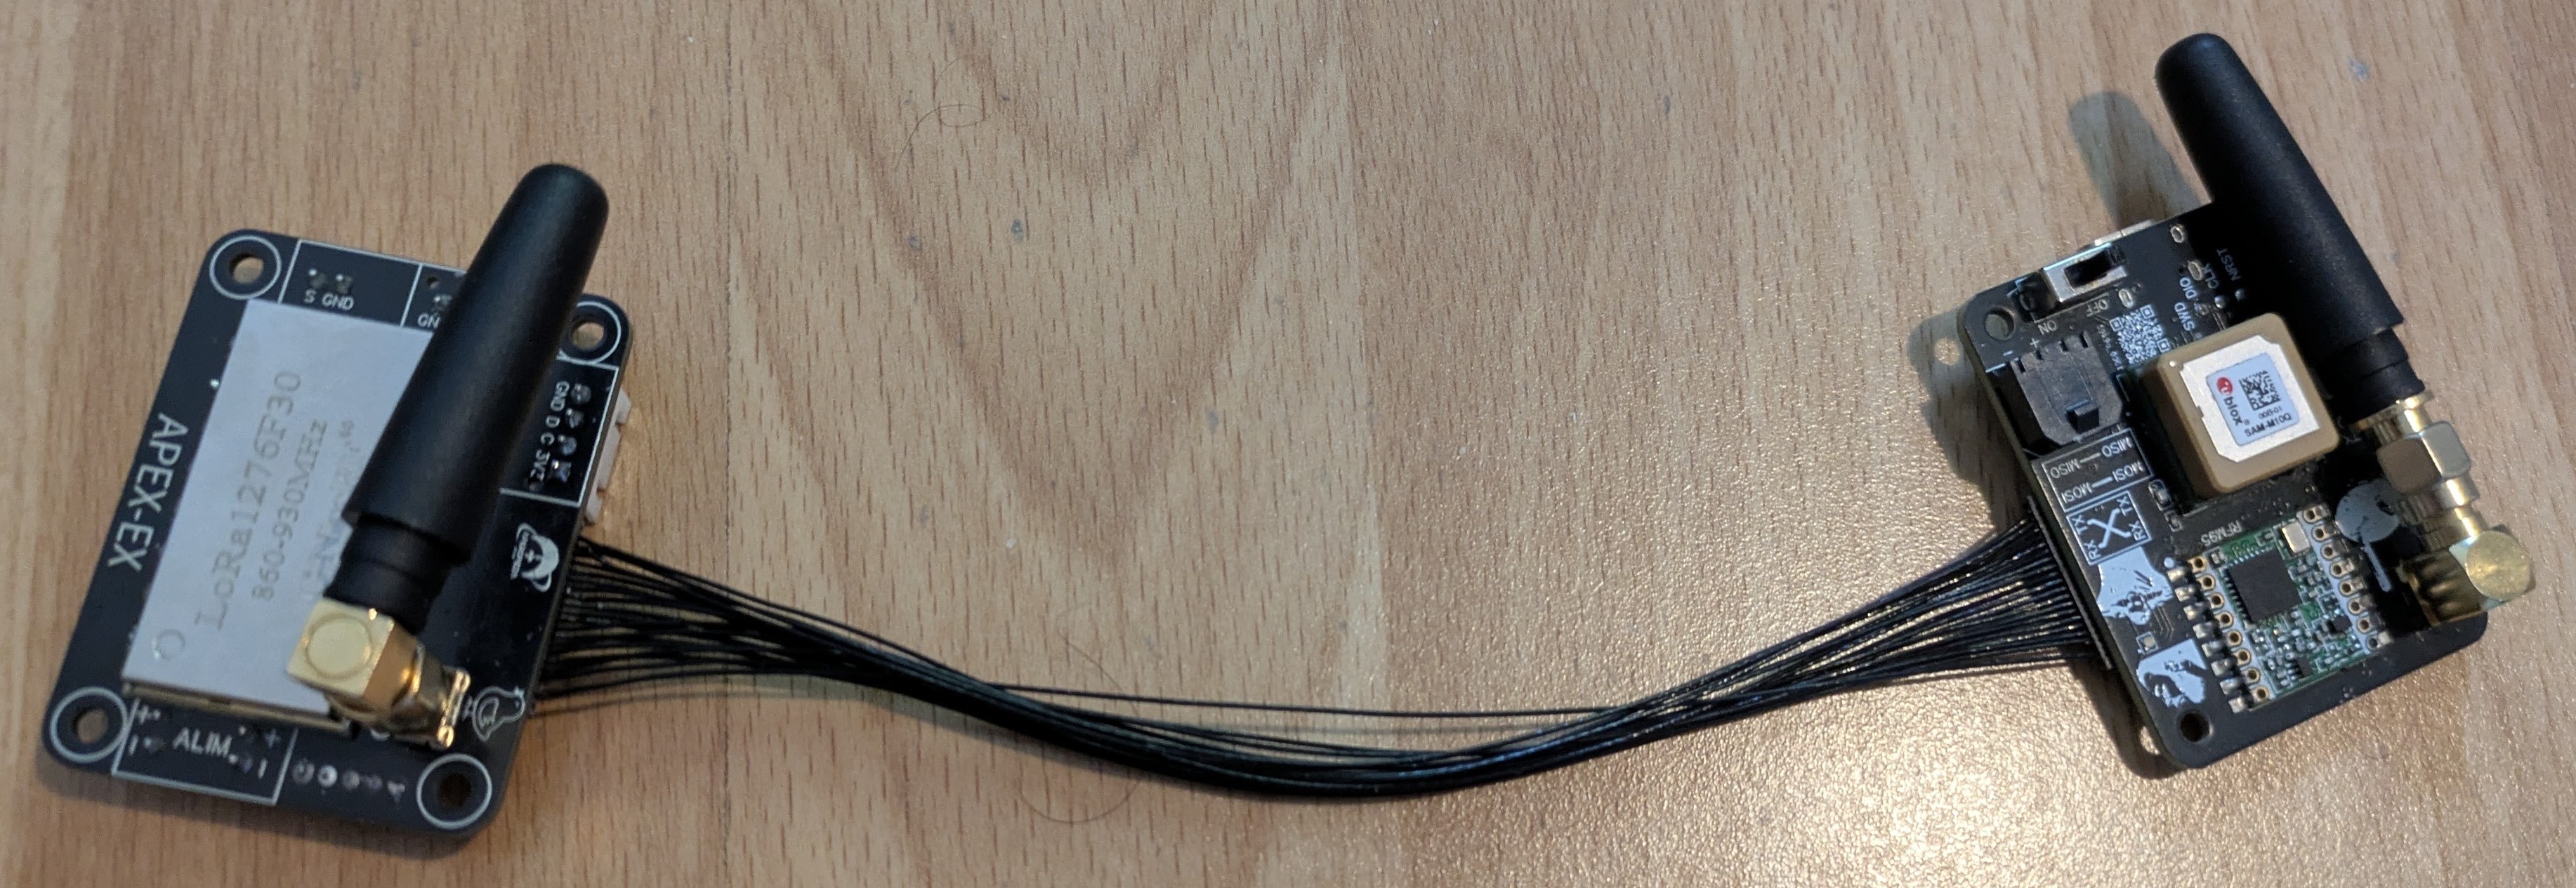
\includegraphics[width=0.8\textwidth]{figures/elec/Apex_ApexEx_2.jpg}
    \caption{Apex et ApexEx branché par le connecteur 20 pins.}
\end{figure}

\newpage

\subsubsection{Système expérimental Apex}

Le système expérimental Apex dans le cadre du projet SP-02 est donc constitué du module \gls{APEX}, de la carte ApexEx et de la
carte Pitot.

\subsubsubsection{Mesure de la vitesse aéronautique}

\hspace*{-\parindent}%
\begin{minipage}{0.25\textwidth}
    \begin{figure}[H]
        \begin{subfigure}{1.0\textwidth}
            \centering
            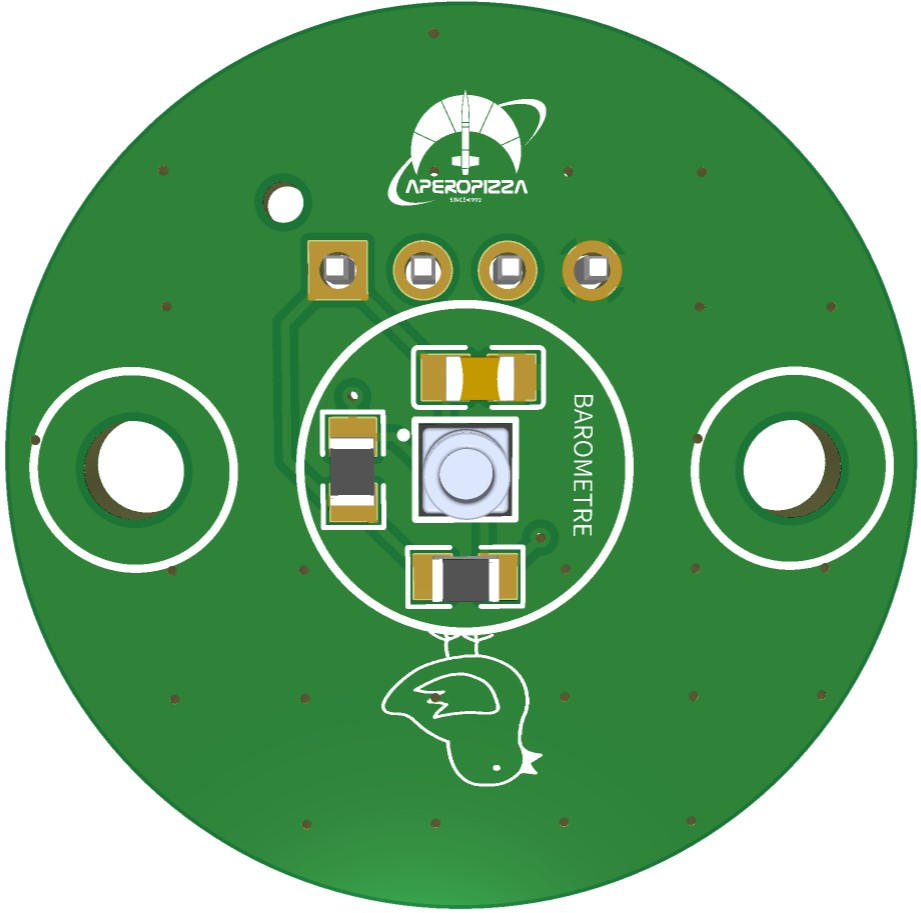
\includegraphics[width=\textwidth]{figures/elec/PCB_Pitot_FRONT.jpg}
            \caption{Vue de face}
            \label{subfig:pitot_front}
        \end{subfigure}
        \begin{subfigure}{1.0\textwidth}
            \centering
            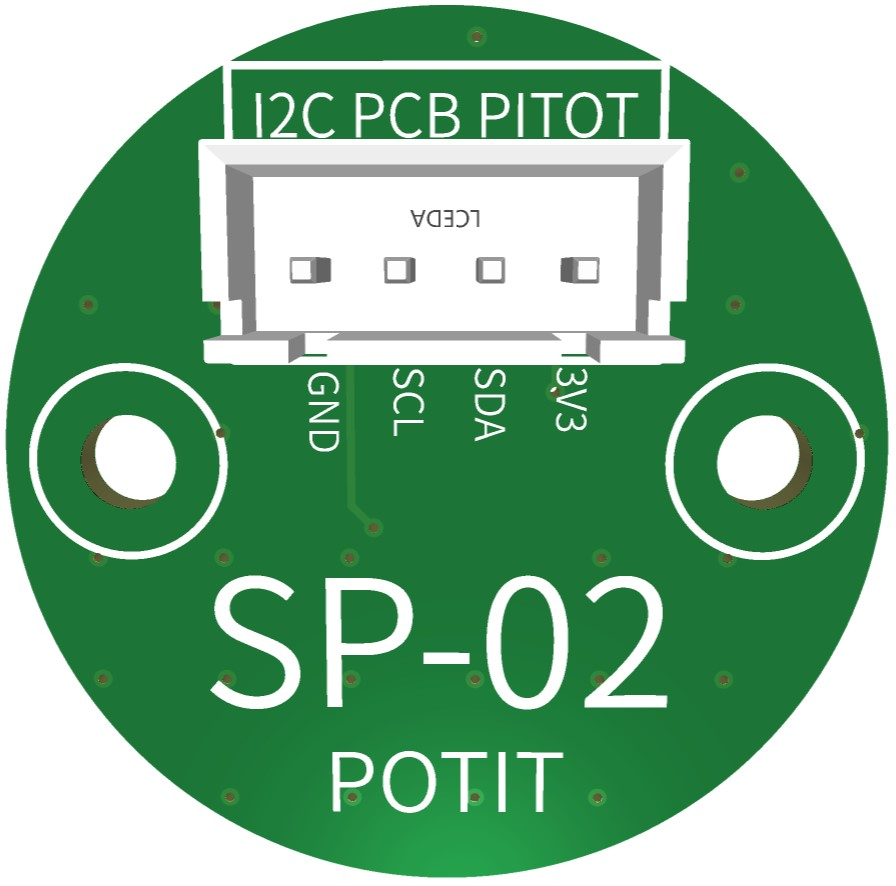
\includegraphics[width=\textwidth]{figures/elec/PCB_Pitot_BACK.jpg}
            \caption{Vue de dos}
            \label{subfig:pitot_back}
        \end{subfigure}
        \caption{Module Pitot.}
        \label{fig:pitot}
    \end{figure}
\end{minipage}
\hfill
\begin{minipage}{0.65\textwidth}
    La technique de mesure de la vitesse aéronautique utilisée par le module expérimental est la technique dite de la sonde
    Pitot. Elle consiste à mesurer la pression totale au niveau de la pointe de la coiffe du deuxième étage, ainsi que la
    pression statique à l'intérieur du fuselage de la fusée. La différence entre ces deux pressions permet de calculer la vitesse
    de l'air par rapport à la fusée.\\

    $$v_{air} = \sqrt{\frac{2\times\left(P_{t} - P_{s}\right)}{\rho}}$$

    \noindent où $v_{air}$ est la vitesse de l'air par rapport à la fusée, $P_{t}$ est la pression totale et $P_{s}$ est la
    pression statique. La masse volumique de l'air $\rho$ est estimé à partir de l'estimation de l'altitude de la fusée, elle-même
    calculée à partir de la pression statique. \\

    Sachant que la vitesse maximale de la fusée est estimée à \SI{180}{\meter\per\second}, la pression totale maximale peut être
    rapidement majorée à :
    \begin{align*}
        P_t &= \frac{1}{2}\rho v^2 + P_s \\
        &= \frac{1}{2} \times 1.225 \times (180)^2 + P_s \\
        &= 19845 + 101325 \\
        &= 121170 \text{ Pa} \\
        &= 1211.7 \text{ hPa}
    \end{align*}
\end{minipage}

\vspace{0.2cm}

Le baromètre \verb|ILP28SQSW| est capable de mesurer des pressions allant de \SI{260}{\hecto\pascal} à \SI{1260}{\hecto\pascal}
dans un premier mode de fonctionnement, et de \SI{260}{\hecto\pascal} à \SI{4060}{\hecto\pascal} dans un second mode
moins sensible. Il est donc capable de mesurer la pression totale dans la plage de fonctionnement de la fusée.\\

En considérant la plage de fonctionnement du baromètre, l'altitude maximale qui peut être mesurée par le module expérimental est
de l'ordre de \SI{10}{\kilo\meter} et la vitesse maximale mesurable est de l'ordre de \SI{705}{\meter\per\second}.

\vfill

[METTRE PHOTO ASSEMBLAGE POINTE PLUS PITOT]

\vfill

\newpage

\subsubsubsection{Chaines de télémesures}

Comme établi précédemment, la chaîne de télémesure doit permettre de récupérer le flux de données de vol même en cas de perte
d'un étage, et rend possible par la même occasion un suivi de la trajectoire en direct depuis le sol. Aucune modulation ne
satisfait cependant simultanément les exigences contradictoires de débit et de robustesse : l'architecture retenue en associe donc
deux, le \acrshort{LORA}, robuste mais lent, pour les données essentielles à la reconstruction de la trajectoire, et le
\acrshort{FSK}, rapide mais plus sensible au bruit, pour le reste du flux.\\
 
Chaque étage embarque un module par modulation, soit quatre transceivers, tous construits autour de la même puce Semtech
\verb|SX1276| qui supporte nativement les deux. Le plan de fréquences attribue une fréquence par modulation et non par module :
\SI{868}{\mega\hertz} pour les deux liens \acrshort{LORA}, \SI{869.5}{\mega\hertz} pour les deux liens \acrshort{FSK}, cette
sous-bande autorisant une puissance d'émission de \SI{500}{\milli\watt}. La station sol se réduit ainsi à deux récepteurs, mais
deux émetteurs partagent chaque canal : l'accès est organisé par \acrfull{TDM}.

\begin{figure}[H]
    \centering
    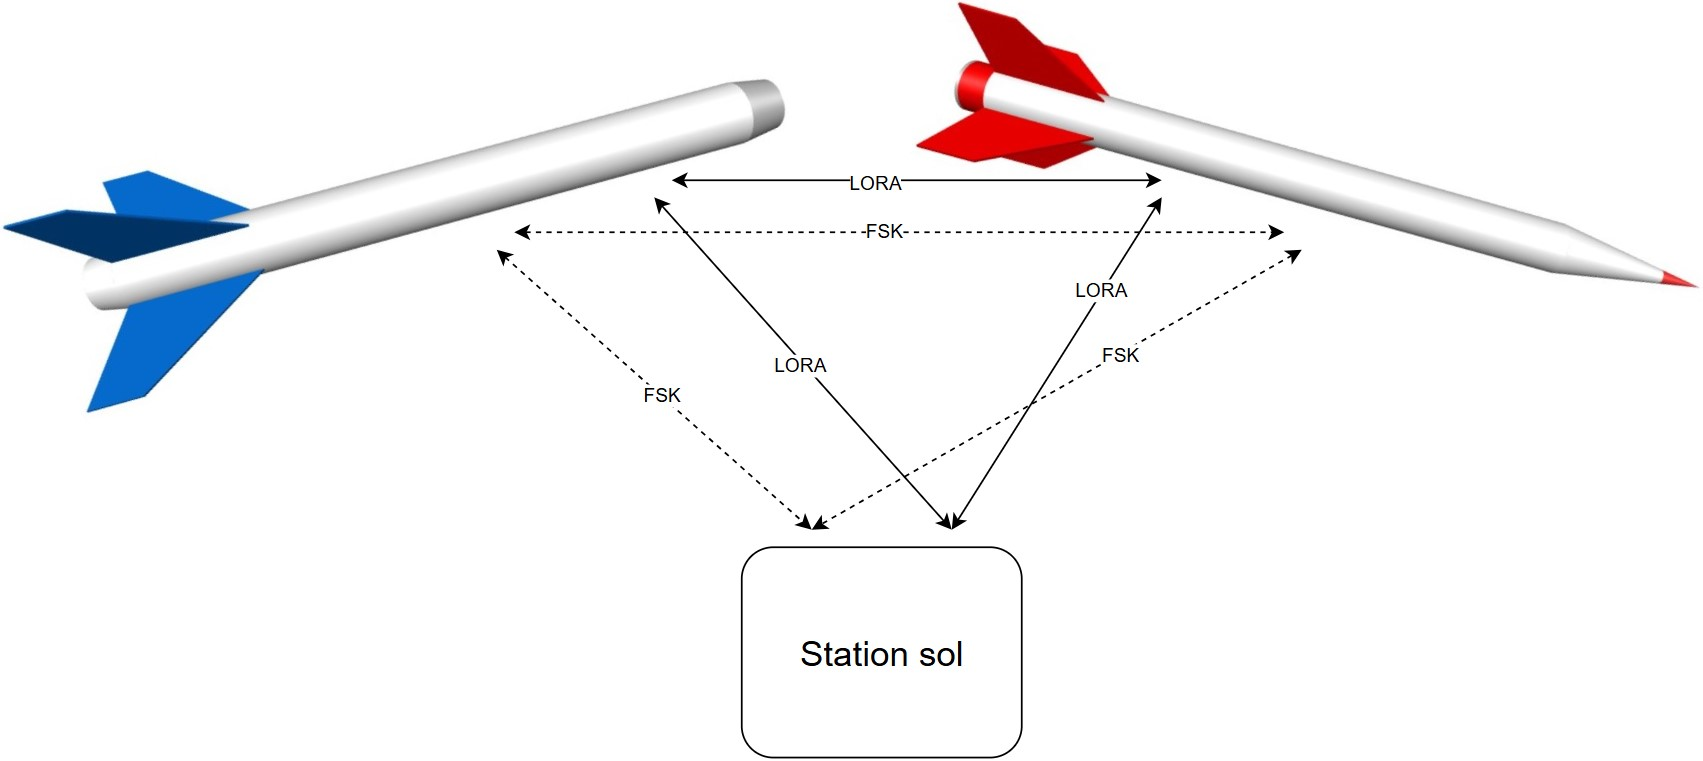
\includegraphics[width=\textwidth]{figures/elec/SP02_telem.jpg}
    \caption{Vue d'ensemble de la chaîne de télémesure}
    \label{fig:telem}
\end{figure}

\paragraph*{Protocole \acrshort{LORA}}
 
Le \acrfull{LORA} est une modulation propriétaire de Semtech reposant sur un étalement de spectre à variation linéaire de
fréquence (\textit{Chirp Spread Spectrum}) : chaque symbole est codé par un \textit{chirp} balayant toute la bande allouée.
Le gain de traitement qui en résulte permet de démoduler un signal dont la puissance est inférieure au niveau de bruit.\\
 
Le débit, fixé par le facteur d'étalement (SF7 à SF12), la bande passante et le taux de codage, reste en revanche limité à
\SI{37.5}{\kilo bit\per\second} au mieux sur le \verb|SX1276|, soit un ordre de grandeur en dessous du flux produit par
l'expérience. Le \acrshort{LORA} ne porte donc qu'un sous-ensemble réduit des données, à cadence réduite, mais constitue le
lien le plus fiable de la chaîne.
 
\paragraph*{Protocole \acrshort{FSK}}
 
Le \acrfull{FSK} code l'information par le décalage de la porteuse autour de sa valeur nominale. Sans étalement de spectre, il
ne bénéficie d'aucun gain de traitement, mais accepte des débits bien supérieurs : jusqu'à \SI{300}{\kilo bit\per\second} sur le
\verb|SX1276|, largement de quoi couvrir les \SI{101.6}{\kilo bit\per\second} produits par l'expérience. La sensibilité,
d'environ \SI{-118}{\dBm} à bas débit, se dégrade toutefois à mesure que celui-ci augmente.\\
 
La chaîne met en œuvre la variante \acrfull{GFSK}, dans laquelle le signal modulant est mis en forme par un filtre gaussien. Ce
filtrage supprime les discontinuités de phase responsables de l'étalement spectral à débit et complexité de démodulation inchangés.
 
\newpage


\hspace*{-\parindent}%
\begin{minipage}{0.45\textwidth}
    \paragraph*{Module SX1276X, RFM95W et LORA1276F30}
    Les quatre transceivers reposent sur la puce Semtech \verb|SX1276|, transceiver sub-gigahertz couvrant la bande
    \SIrange{137}{1020}{\mega\hertz}, piloté par bus \acrshort{SPI} et supportant les modulations \acrshort{LORA}, \acrshort{FSK},
    \acrshort{GFSK} et \acrshort{OOK}. Deux modules du commerce fondés sur cette puce ont été retenus : le \verb|RFM95W| de
    HopeRF, qui se limite au front-end radio du composant, et le \verb|LoRa1276F30| de NiceRF, qui y ajoute un amplificateur de
    puissance en émission et un amplificateur faible bruit en réception.
\end{minipage}
\hfill
\begin{minipage}{0.5\textwidth}
    \begin{table}[H]
        \centering
        \begin{tabular}{lcc}
            \hline
            & \verb|RFM95W| & \verb|LoRa1276F30| \\
            \hline
            Modulation & \acrshort{LORA} & \acrshort{GFSK} \\
            Fréquence & \SI{868}{\mega\hertz} & \SI{869.5}{\mega\hertz} \\
            Puissance maximale & \SI{20}{\dBm} & \SI{27}{\dBm} \\
            Puissance retenue & \SI{25}{\milli\watt} & \SI{500}{\milli\watt} \\
            Sensibilité & \SI{-148}{\dBm} & \SI{-139}{\dBm} \\
            \hline
        \end{tabular}
        \caption{Caractéristiques des modules de télémesure}
        \label{tab:modules_telemesure}
    \end{table}
\end{minipage}
 
\subsubsubsection{Communication avec le séquenceur}

La liaison entre le séquenceur et le module expérimental doit permettre au premier d'informer le système \gls{APEX} de son état. Les
algorithmes de calcul de trajectoire peuvent ainsi sélectionner les modèles et les paramètres de vol adaptés à la phase en cours. Elle
permet en outre, après le vol, de reconstruire la chronologie des actions du séquenceur, de vérifier qu'il a bien rempli sa mission et de
mesurer le décalage temporel entre chacune de ses commandes et la réponse effective de la fusée.\\

En raison d'une contrainte d'occupation du bus \acrshort{UART} (détaillée en section~\ref{subsubsubsec:apex_pb_bus}), le système
\gls{APEX} doit se placer dans une configuration particulière pour que son microcontrôleur soit effectivement relié au séquenceur. Deux
approches ont été envisagées.\\

\begin{itemize}
    \item \textbf{Interrogation périodique.} \gls{APEX} établit la connexion à intervalle régulier et interroge le séquenceur, qui lui
    transmet en réponse les actions effectuées depuis la requête précédente. Simple à mettre en œuvre, cette approche ne permet pas de
    suivre les changements d'état du séquenceur en temps réel. Elle impose surtout de fixer une cadence d'interrogation : suffisamment
    élevée pour ne pas perdre d'information, mais suffisamment faible pour ne pas saturer le bus \acrshort{UART}. Le séquenceur doit par
    ailleurs conserver en mémoire les actions accumulées entre deux requêtes. Cette mémoire tampon appartient ici au fonctionnement
    nominal : sa taille, configurée dans le séquenceur, doit être dimensionnée en fonction de la cadence d'interrogation, elle-même
    configurée dans \gls{APEX}. Un tel couplage entre deux paramètres appartenant à deux sous-systèmes distincts est fragile. Tout 
    ajustement de la cadence impose de revalider le dimensionnement du tampon, et un sous-dimensionnement se traduit directement par une
    perte d'événements.\\

    \item \textbf{Notification par \acrshort{GPIO}.} À chaque action, le séquenceur signale l'événement à \gls{APEX} en modifiant l'état
    d'une broche \acrshort{GPIO} dédiée. \gls{APEX} détecte cette transition, établit la connexion et interroge le séquenceur pour
    récupérer les actions concernées. Plus complexe à mettre en œuvre, cette approche suit les changements d'état en temps réel et
    supprime le choix d'une cadence d'interrogation. Le séquenceur maintient également dans cette approche une liste des actions en
    mémoire, mais celle-ci ne relève plus du fonctionnement nominal : elle n'est sollicitée qu'en cas de défaillance ponctuelle,
    matérielle ou logicielle, empêchant \gls{APEX} de répondre à une notification. Cette liste est vidée à chaque échange abouti et son
    dimensionnement n'est plus lié à un paramètre extérieur au séquenceur.
\end{itemize}

La seconde approche a été retenue. Outre le suivi en temps réel, elle supprime le couplage entre la cadence d'interrogation et le
dimensionnement du tampon plutôt que de le déplacer, et offre un comportement dégradé plus sûr : le tampon n'intervenant qu'en cas de
défaillance, une anomalie ponctuelle retarde la remontée des événements sans les perdre. \\

Cette connexion se matérialise par deux connecteurs :
\begin{itemize}
    \item \verb|UART_SEQ_EXP| : un connecteur à 4 broches (3V3, RX, TX, GND) branché côté séquenceur sur le connecteur \verb|UART|
    (voir figure \ref{fig:synopsis_sequ}) et côté \gls{APEX} sur le connecteur \verb|UART| du module ApexEx (voir figure
    \ref{fig:zoom_syno_apex}).

    \item \verb|IRQ_SEQ_EXP| : un connecteur à 2 broches (IRQ, GND) branché côté séquenceur sur le connecteur \verb|OUT_OPTO_N1|
    (voir figure \ref{fig:synopsis_sequ}) et côté \gls{APEX} sur le connecteur \verb|IRQ| du module ApexEx (voir figure
    \ref{fig:zoom_syno_apex}).
\end{itemize}

\newpage

\subsubsubsection{Interface avec le système de caméra embarqué}

L'interface entre \gls{APEX} et le système de caméra embarqué se réduit à un connecteur à deux points, portant une ligne
d'interruption et la masse. Le rôle d'\gls{APEX} se limite à émettre un stimulus sur cette ligne à un instant donné, soit sur
réception d'un ordre transmis par la chaîne de télémesure, soit de manière autonome. Ce stimulus est interprété en aval par le
système de caméra, qui en déduit l'activation ou l'extinction des caméras.\\

Le recours à un ordre transmis depuis le sol appelle une précision : le projet interdit en principe toute liaison de télémesure
montante. Cette commande ne fait pas exception à la règle sur le fond, car elle n'est ni émise ni traitée en vol. Elle n'intervient
qu'une fois la fusée au sol et l'ensemble des opérations pyrotechniques achevé, si bien qu'elle ne peut influer ni sur le
déroulement du vol ni sur la sécurité des opérations.

\subsubsubsection{Encombrement des bus de communications}
\label{subsubsubsec:apex_pb_bus}

La liaison entre les cartes Apex et ApexEx transite par un unique connecteur vingt points, dont le nombre de lignes limité a
imposé des arbitrages sur deux bus de communication.

\paragraph*{UART}
Le premier concerne l'\acrshort{UART}. Le connecteur ne met à disposition qu'une seule liaison, alors que deux interfaces la
requièrent côté ApexEx : la centrale inertielle \verb|WT901B| et la connexion avec le séquenceur. Un multiplexeur analogique
\verb|TMUX1136DGSR| a donc été inséré sur ce bus. Ce composant regroupe deux commutateurs 2:1 bidirectionnels, dont les entrées de
sélection sont réunies sur une même broche \acrshort{GPIO} du microcontrôleur : les lignes TX et RX basculent ainsi simultanément
vers l'une ou l'autre des deux interfaces, qui deviennent de ce fait mutuellement exclusives. À un instant donné, le
microcontrôleur ne peut dialoguer qu'avec un seul des deux périphériques.

\paragraph*{I2C}
Le second concerne l'\acrshort{I2C}. Les baromètres retenus ne proposent qu'un jeu d'adresses restreint, insuffisant pour distinguer
sur un même bus les deux exemplaires présents sur ApexEx et celui embarqué sur Apex. Un multiplexeur \verb|PCA9540BDP| a donc été
ajouté : ce composant répartit le bus amont sur deux segments aval dont un seul est actif à la fois, ce qui permet à des
périphériques de même adresse de coexister. Contrairement au précédent, il ne requiert aucune ligne de commande dédiée puisqu'il
est lui-même adressé en \acrshort{I2C}, la voie active étant sélectionnée par écriture dans son registre de contrôle. Sa mise sous
tension le laisse par ailleurs dans un état où aucune voie n'est sélectionnée, ce qui garantit l'absence de conflit d'adresse tant
que le logiciel n'a pas explicitement configuré le bus.

\newpage
